%---- Sample WMSU BSMATH BEAMER template ------
%---- Begin editing after PREAMBLE END at line 77------
%---- Created by: Christle Jude L. Maquilan - April 2022 --
%---- @jmaq03.jm@gmail.com -----

\documentclass[xcolor=dvipsnames,envcountsect]{beamer}

%------------------------------------------------
%------------------------------------------------
%------------------------------------------------
%------------------------------------------------
%------------------------------------------------
%----------▼▼▼▼▼ START PREAMBLE ▼▼▼▼▼----------

%-------- theme --------
\usetheme{Madrid}

%-------- color --------
\definecolor{crimsonred}{RGB}{153,0,0} % Official RGB code for Crimson Red
\usecolortheme[named=crimsonred]{structure}
%-------- set color of 'example block' to crimson theme --------
\setbeamercolor{block body example}{bg=white}
\setbeamercolor{block title example}{fg=white, bg=red!50!black}

%-------- font --------
\setbeamerfont{structure}{family=\rmfamily,series=\bfseries}
\usefonttheme[stillsansseriftext]{structurebold}
\setbeamerfont{section in head/foot}{size=\tiny}

%-------- misc structure --------
\useoutertheme[footline=authortitle,subsection=false]{miniframes}
\useinnertheme{rounded}
\addtobeamertemplate{block begin}{}{\justifying}
\newtheorem{remark}[theorem]{Remark}
\renewcommand{\indent}{\hspace*{2em}}
\setbeamertemplate{theorems}[numbered]
\setbeamertemplate{caption}[numbered]
\usepackage[justification=centering]{caption}
\renewcommand{\qedsymbol}{$\blacksquare$}

%-------- packages to be used -------
\usepackage{amsmath,amsfonts,amssymb,amscd,amsthm}
\usepackage{graphicx,xcolor,comment}
\usepackage{mathrsfs} 
\usepackage{multirow}
\usepackage{array}
\usepackage{hyperref}
\usepackage{multicol}
\usepackage{ragged2e}
\usepackage{caption}
\usepackage[french]{babel}
\usepackage{rotating}
\usepackage{enumerate}
\usepackage{tikz}
\usepackage{bm}
\usepackage{csquotes}
\usepackage{wrapfig}

%-------- for bibliography -----------------
\usepackage{biblatex}
\setbeamertemplate{bibliography item}{\insertbiblabel}
\addbibresource{References.bib}
\setbeamertemplate{frametitle continuation}{\frametitle{\color{white}Bibliographie}}

%-------- WMSU Backgound -------------------
%\usebackgroundtemplate{%
%	\tikz[overlay,remember picture] \node[opacity=0.02, at=(current page.center)] {
%		
\includegraphics[height=4.5in,width=4.5in]{./Figures/WMSU LOGO.png}};
%}

%----------▲▲▲▲▲ PREAMBLE END ▲▲▲▲▲----------
%------------------------------------------------
%------------------------------------------------
%------------------------------------------------
%------------------------------------------------
%------------------------------------------------

%---------START EDITING HERE---------------------
\title[Études des systèmes GNSS des smartphones]{Études des systèmes GNSS des smartphones}

\author [Noë Charlier]{\textbf{Noë Charlier}}

\institute[Lycée Paul Constans] {\emph{Professeurs: }\textbf{C. Delacour, M. Petitcuenot}\\[1em]
	Classe préparatoire aux grandes écoles\\PT\\Lycée Paul Constans\\[1em]

\includegraphics[scale=0.4]{./Figures/logo Paul Constans.jpg}}

\date[2022 - 2023]{\footnotesize TIPE - \textbf{2022, 2023}}
%--------- START DOCUMENT ------------------
\begin{document}
	
\begin{frame}{\titlepage}\end{frame}
\begin{frame}{\frametitle{Sommaire}\tableofcontents}\end{frame}
%--------- Sujet et Domaine ----------------------
\section{Introduction}
\begin{frame}
	\frametitle{Introduction}
		\justifying
		\textit{Besoin grandissant de solution GNSS:}
		\begin{figure}
			\centering
			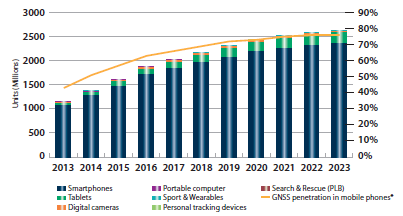
\includegraphics[scale=0.8]{./Figures/stats.png} \\
			\caption {Appareils GNSS par plate-forme. \cite{marketreport}}
		\end{figure}
\end{frame}
\begin{frame}
	\frametitle{Définition GNSS}
		\justifying
		\textbf{GNSS:} \textit{Global Navigation Satellite System} (Système de navigation par satellite global)\\
		Constellation de satellites permettant de localiser un point sur la Terre.
		\begin{figure}
			\centering
			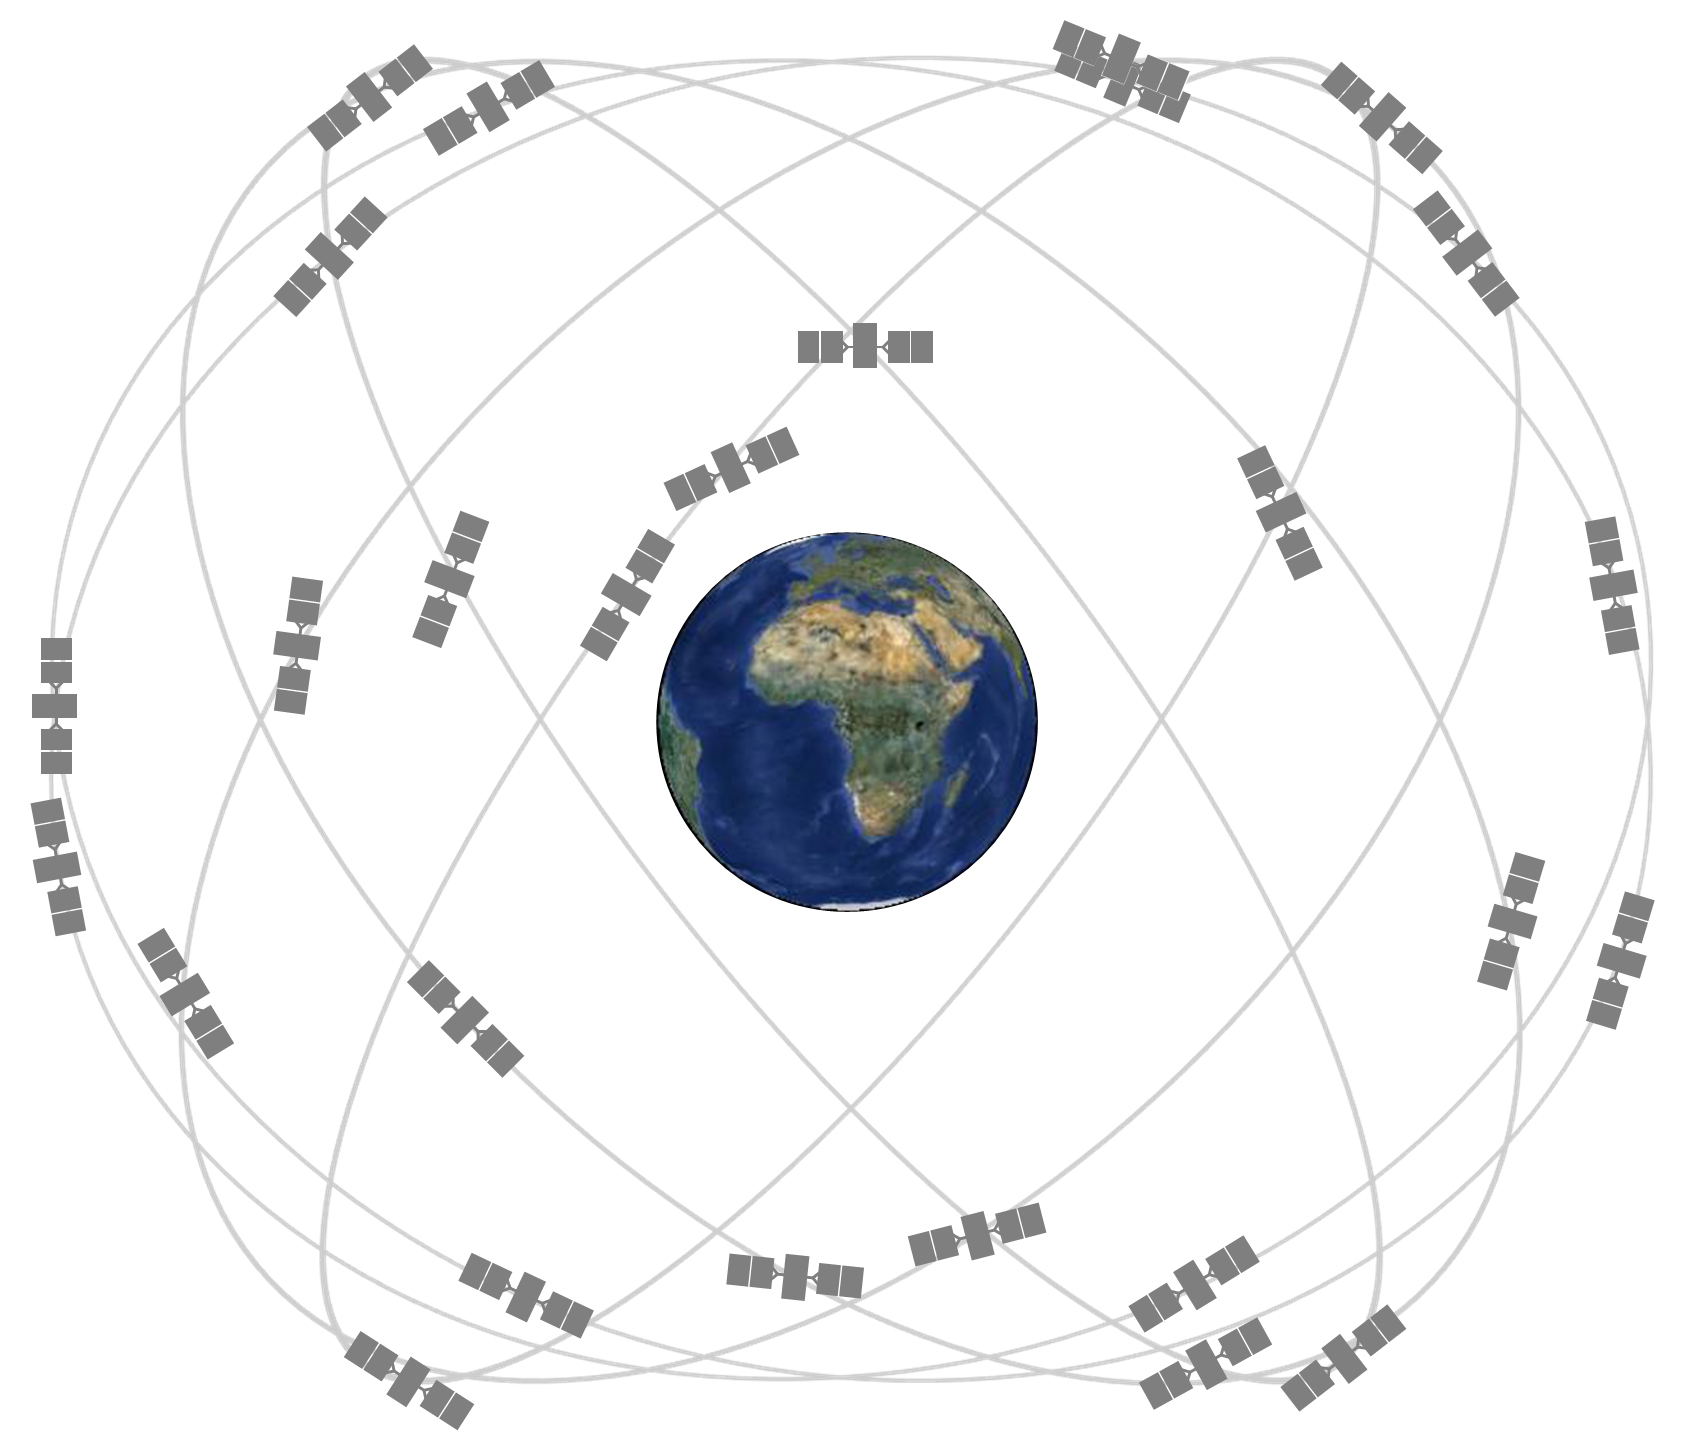
\includegraphics[width=0.3\textwidth]{./Figures/constellation.jpg} \\
			\caption {Système de navigation par satellite global. \cite{cons}}
		\end{figure}
\end{frame}

\begin{frame}
	\frametitle{Fonctionnement du GPS}
	\justifying
	\begin{columns}

		\begin{column}{0.5\textwidth}
			\begin{figure}
				\centering
				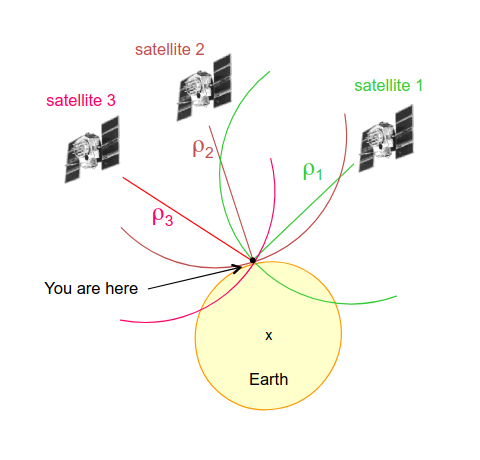
\includegraphics[width=0.9\textwidth]{./Figures/ENS_gnss.png} \\
				\caption {Fonctionnement du GPS. \cite{ens}}
			\end{figure}
		\end{column}

		\begin{column}{0.5\textwidth}
			Une sphère de rayon $\rho_1 = (\Delta t_1 \cdot c) $ \\
			3 satellites, intersection des 3 sphères.
			\newline
			Et donc {\footnotesize$\rho_s^s = \sqrt{(X^s-X_r)^2 + (Y^s-Y_r)^2 + (Z^s-Z_r)^2}$} \\
			Avec:
			\begin{itemize}
				\item $X^s, Y^s, Z^s$ : coordonnées du satellite $s$ ;
				\item $X_r, Y_r, Z_r$ : coordonnées du récepteur.
			\end{itemize}
		\end{column}

	\end{columns}

\end{frame}

\begin{frame}
	\frametitle{Sources d'incertitude}
	\justifying
	\begin{itemize}
		\item Les horloges des satellites et des récepteurs ne sont pas synchronisés. ($\delta t$)
		\item Réfraction lors de la propagation dans l’atmosphère :
		\item \begin{enumerate}
			\item Troposphérique (dépend de la température et de la pression atmosphérique) ($T_r^s$)
			\item Ionosphérique (dépend de la densité ionique) ($I_r^s$)
		\end{enumerate}
	\end{itemize}
	Modèle plus complet :
	\begin{equation}
		\boxed{R_r^s = \rho_r^s + c\delta t + T_r^s + I_r^s + ...}
	\end{equation}
\end{frame}
\begin{frame}
	\framesubtitle{Précision des orbites}
	\justifying
	Les systèmes GNSS sont basés sur des orbites prédites émises par les satellites. \\
	Ces \textbf{éphémérides} doivent donc être très précises. {\tiny(Perturbation gravitationnelle (cf. Annexe), radiation solaire ...)} \\
	\begin{figure}
		\centering
		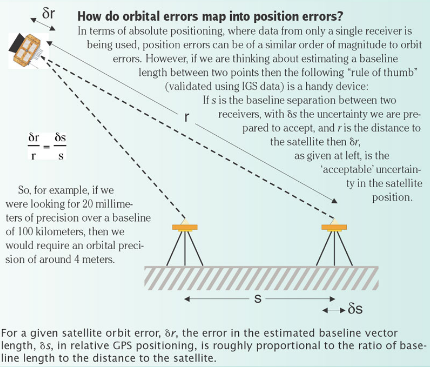
\includegraphics[width=0.4\textwidth]{./Figures/ENS_gnss2.png} \\
		\caption {Précision des orbites. \cite{ens}}
	\end{figure}
	{\small	\textit{Il existe aussi des services qui recalculent les éphémérides apostériori. (eg. IGN)}}
\end{frame}
%---------- DEFINITION/PRELIMINARY ---------------------
\section{L'ionosphère}
\begin{frame}
	\frametitle{Définition}
	\begin{columns}
	    \justifying
		\begin{column}{0.5\textwidth}
	    	\textbf{L'ionosphère :} 
			L'ionosphère est la couche de l'atmosphère située entre 60 et 1000 km d'altitude.
			Elle est constituée de particules chargées électriquement, les ions, qui sont en mouvement.
		\end{column}
		\begin{column}{0.5\textwidth}
			\begin{figure}
				\centering
				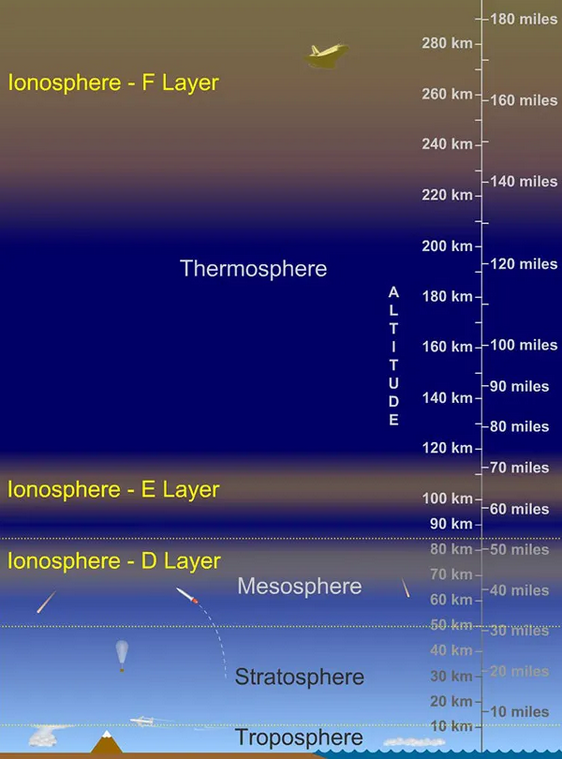
\includegraphics[width=0.7\textwidth]{./Figures/iono_ucar.png}
				\caption {Régions de l'ionosphère \cite{ucar}}	
			\end{figure}
		\end{column}	
	\end{columns}
\end{frame}
\begin{frame}
	\frametitle{Impact sur la propagation}
		\justifying
		\begin{columns}
			\begin{column}{0.5\textwidth}
				\textbf{Impact sur la propagation :} 
				\begin{itemize}
					\item \textbf{Propagation directe} - La propagation directe est la propagation d'une onde radio entre deux points sans interaction avec l'ionosphère.
					\item \textbf{Propagation diffusée} - La propagation diffusée est la propagation d'une onde radio entre deux points avec interaction avec l'ionosphère.
				\end{itemize}
			\end{column}
			\begin{column}{0.5\textwidth}
				\begin{figure}
					\centering
					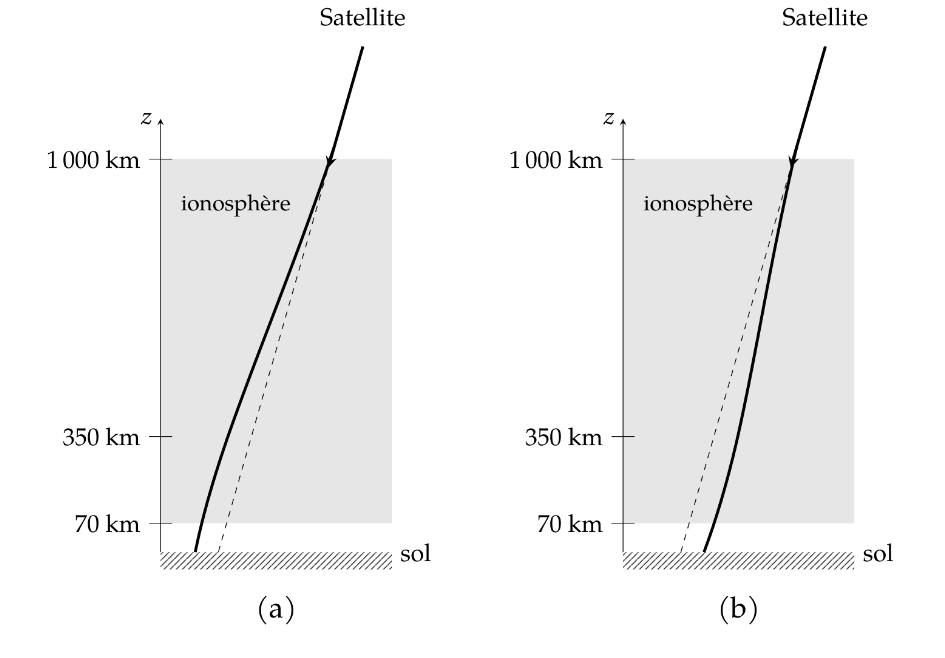
\includegraphics[width=0.7\textwidth]{./Figures/iono_e3a.png}
					\caption {Propagation directe et diffusée \cite{e3a}}	
				\end{figure}
			\end{column}
	\end{columns}
\end{frame}
\begin{frame}
	\framesubtitle{TEC}
	\textit{Total Electron Content} (Contenu total d'électrons)\\
	\textbf{TEC:} Quantité d'électrons présents dans une couche de l'ionosphère.\\
	
\end{frame}

%----------- MAIN RESULTS ------------------------------
\section{Objectifs \& Expérimentations}
\begin{frame}{Expérimentations (\& Simulations numérique) et Objectifs}
        \textbf{Expérimentations:} 
	    \begin{itemize}
            \item \textbf{Etude du lien entre SID et précision GPS} - Capteur GPS, et récepteur basse fréquence
        \end{itemize}
        \textbf{Modélisations:} 
	    \begin{itemize}
            \item \textbf{Système GPS réduit} - Modélisation d'un système de résolution GPS afin de lien les résultats expérimentaux.
        \end{itemize}
	%\indent To see this, consider graphs $G_{1}=P_{3}, G_{2}=P_{4}$, and $G_{3}=C_{8}$ in Figure \ref{3.1}.
\end{frame}
\section{Positionnement thématique}
\begin{frame}
	\frametitle{Positionnement thématique}
		\justifying
		%\newline
		%\newline
		\textbf{Positionnement thématique:}
		\begin{itemize}
            \item \textbf{Physique} - Physique Interdisciplinaire
            \item \textbf{Sciences Industrielles} - Traitement du Signal \& Électronique
            \item \textbf{Informatiques} - Informatique Pratique
            \item \textbf{Mathématiques} - Mathématiques Appliquées
        \end{itemize}
\end{frame}

\begin{frame}
	\centering
	\begin{block}
		\scshape
			\begin{center}
				\Huge\emph{Des Questions ?}
			\end{center}
	\end{block}
\end{frame}

\appendix
\begin{frame}
	\frametitle{Bibliographie}
	\printbibliography
\end{frame}

\section{Annexe 1}
\begin{frame}
	\frametitle{Modélisation, perturbation gravitationnelle}
	
\end{frame}
%--------- THANK YOU Text ------- texlive-most -------------------
%----------------------------------------------------
\end{document}
